\documentclass[11pt,a4paper]{ltjsarticle}
\usepackage{luatexja-fontspec}
\usepackage{geometry}
\usepackage{booktabs}
\usepackage{array}
\usepackage{multirow}
\usepackage{enumitem}
\usepackage{graphicx}
\usepackage{amsmath}
\usepackage{fancyhdr}
\usepackage{xcolor}
\usepackage{tcolorbox}
\usepackage{hyperref}

\geometry{margin=24mm}
\setmainjfont[BoldFont=Hiragino Kaku Gothic ProN]{Hiragino Mincho ProN}
\setsansjfont{Hiragino Kaku Gothic ProN}
\setmonofont{Menlo}
\hypersetup{colorlinks=true, linkcolor=blue!55!black, urlcolor=blue!55!black}

\pagestyle{fancy}
\fancyhf{}
\lhead{研究進捗報告}
\rhead{2026 年 6 月 14 日}
\cfoot{\thepage}
\renewcommand{\headrulewidth}{0.2pt}

\newcommand{\rk}{\textrm{Recall@}K}
\setlist{nosep}

\begin{document}

\begin{center}
{\sffamily\large 物理モデルの自動構築：データベースの拡大・層化分割・\\テストケースの再生成と評価}
\end{center}
\vspace{0.3em}
\hfill 作成者：M2\ 一洋
\vspace{0.8em}

%======================================================================
\section{前回ゼミ（2026-05-19）の到達点と宿題}
%======================================================================
\textbf{研究の目的}：科学文献から数式を集めておき、「どんな物理モデルを作りたいか」（説明文と入出力変数）を入力すると、そのモデルを構成するのに必要な\textbf{数式の集合}を、まず文章の類似度で候補を絞り、次に\textbf{数式どうしの変数の共有関係から作ったグラフ特徴量}を\textbf{多層パーセプトロン（MLP、単純な順伝播型ニューラルネットワーク）}で評価して順位付けし、提示する。前回ゼミまでの到達点は次のとおりである。

\begin{itemize}[leftmargin=1.5em]
  \item 科学論文 39 報の PDF を大規模言語モデル（Gemini 2.5 Pro）に読ませて数式を抽出し、近隣分野の基礎式も同じ大規模言語モデルに生成させて、\textbf{3{,}244 式}・訓練ケース \textbf{1{,}338 件}を構築した。
  \item \textbf{本手法（グラフ特徴量 ＋ MLP）}と、外部手法である\textbf{大規模言語モデル（LLM）による直接生成}、および文章類似度だけの古典的検索を比較し、複数文献にまたがるケースで本手法が最も良い結果を示した。
  \item \textbf{宿題（先生方からのご指摘）}：先生方から次の 3 点をご指摘いただいた。(1) 関連性の低い数式まで広く集めることが、本当に予測精度の向上に効くのかを実験で確かめること。(2) 論文 PDF をどのように収集したのかを明記すること。(3) 数式が少なく代数方程式（微分を含まない式）に偏ったテストケースの作り方を是正すること。
\end{itemize}

%======================================================================
\section{今回の進捗（要約）}
%======================================================================
前回の宿題に沿って、データの収集・分割・評価を一通りやり直した。要点は次の 6 つである。

\begin{enumerate}[leftmargin=1.8em]
  \item \textbf{データベースの拡大}：分野ごとに論文を新たに収集し、収録数式を 3{,}244 $\to$ \textbf{11{,}146 式}、訓練ケースを 1{,}338 $\to$ \textbf{2{,}838 件}に増やした（\S\ref{sec:db}）。
  \item \textbf{訓練／テストの層化分割}：数式数・入出力変数数・ソース数の\textbf{分布が訓練側とテスト側でそろう}ように分割した。検証用データは訓練側から別に取り分け、分割を変えて 10 回繰り返し評価した（\S\ref{sec:split}）。
  \item \textbf{テストケースの再生成}：前のケースは「数式が最大 4 式と少なく、代数方程式が半分を占める」という偏りがあった。そこで\textbf{加藤先生にご指摘いただいた手順}でケースを作り直した（\S\ref{sec:dae}）。
  \item \textbf{API による再現可能な実装}：論文用の実験はデスクトップ／Web アプリではなく\textbf{API 経由のスクリプト}で行えるようにした（\S\ref{sec:api}）。
  \item \textbf{データ拡張の影響を除いた評価と特性別分析}：水増し用のケースを除いた実験と、最難の DAE のみの実験を行い、\textbf{数式数・ソース数・入力変数数で性能がどう変わるか}を調べた（\S\ref{sec:eval}）。
  \item \textbf{評価指標の見直し}：Recall@3 を、正解式数 $K$ に窓幅を合わせた \textbf{Recall@$K$} に変えた（\S\ref{sec:metric}）。
\end{enumerate}

%======================================================================
\section{データベースの拡大}\label{sec:db}
%======================================================================
分野ごとに論文を新たに収集し、数式データベースを拡大した。数式とケースの作り方は 3 通りである。(1) 論文 PDF を大規模言語モデル（Gemini 2.5 Pro）に読ませ、本文中の数式を抽出した（論文 329 報）。(2) 各工学分野の基礎式は、同じ大規模言語モデルに生成させた（32 分野・670 式）。(3) 複数の文献にまたがるケースは、変数を共有する数式の組を規則ベースで機械的に組み立てて作成した（大規模言語モデルは使わない）。これにより収録数式を \textbf{3{,}244 $\to$ 11{,}146 式}（計 361 ソース）、訓練ケースを \textbf{1{,}338 $\to$ 2{,}838 件}に拡大した。ケースの内訳と、正解式数（＝問題の難しさ）の分布を図~\ref{fig:data} に示す。全 2{,}838 件のうち\textbf{正解に 2 式以上を要する複数式ケースが 74.6\%}を占め、複数の式を組み合わせて選ぶ必要があるケースが多い。これが本手法の利点が出やすい状況である。

\begin{figure}[h]\centering
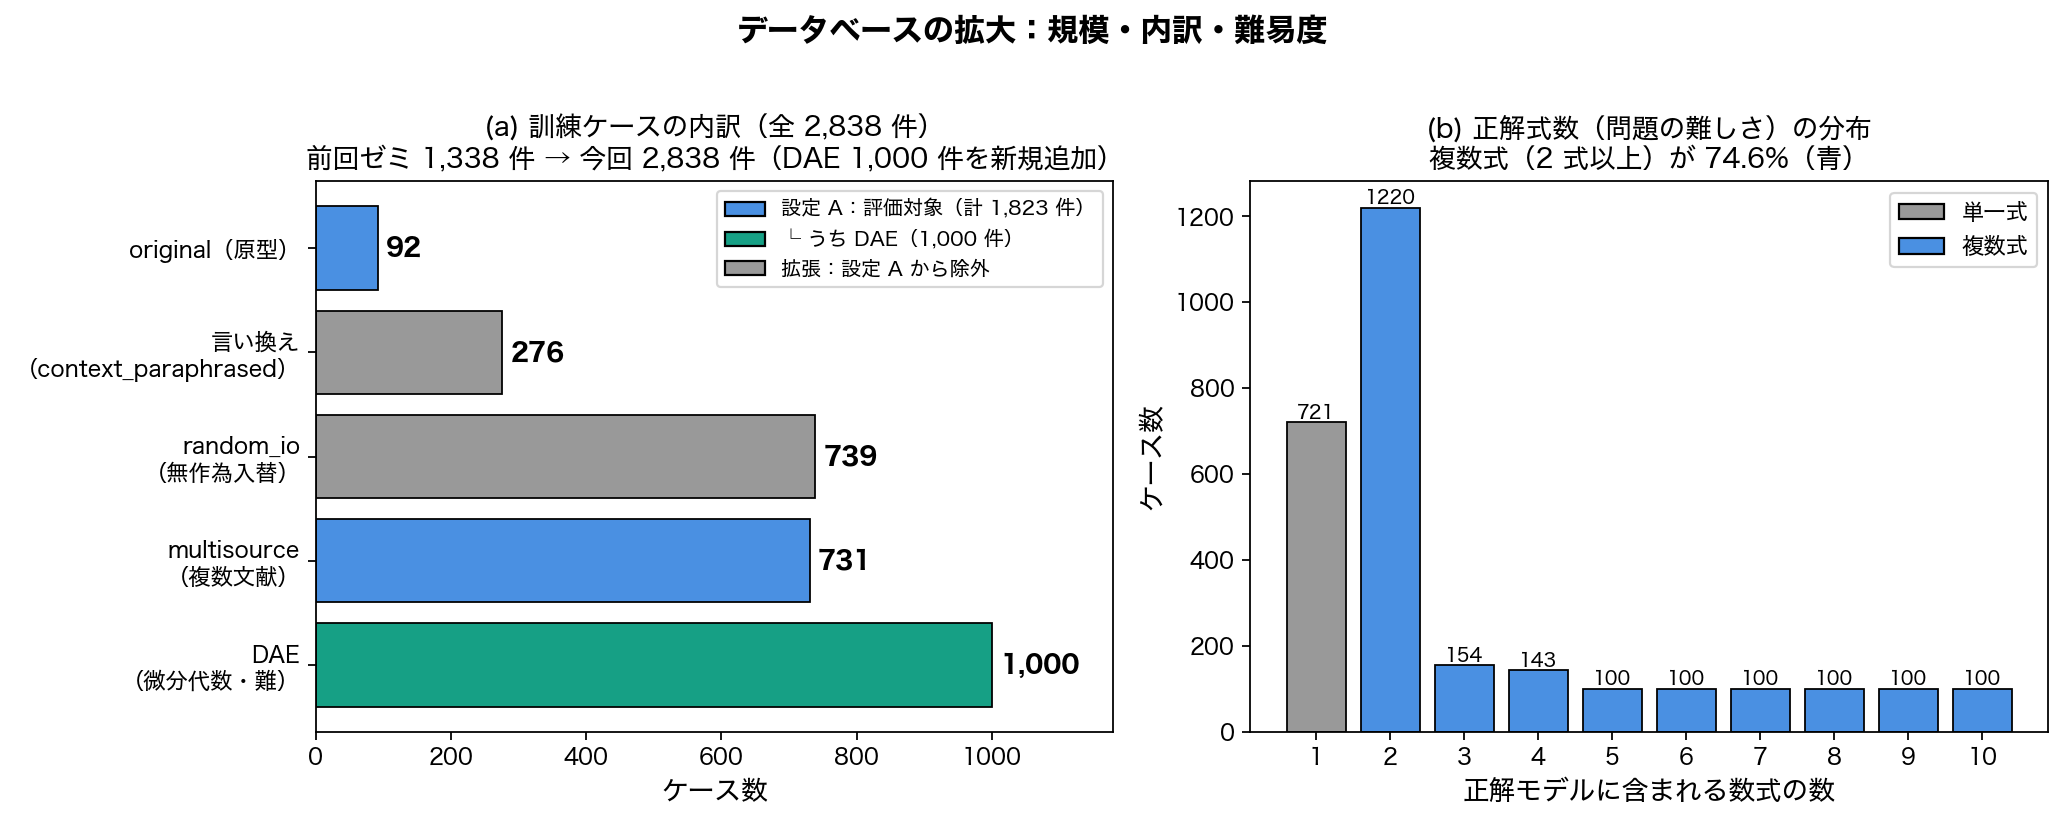
\includegraphics[width=\linewidth]{figures/fig_strat_dataset.png}
\caption{(a) 訓練ケース 2{,}838 件の内訳（DAE 難ケース 1{,}000 件を新規追加）。評価の設定 A（\S\ref{sec:eval}）は原型・複数文献・DAE の 1{,}823 件（$92+731+1{,}000$）。(b) 正解式数の分布：複数式（2 式以上、青）が 74.6\%。}
\label{fig:data}
\end{figure}

%======================================================================
\section{訓練／テストの層化分割}\label{sec:split}
%======================================================================
評価が分割の偏りに左右されないよう、次の 2 点を満たす分割を用いた。

\begin{itemize}[leftmargin=1.5em]
  \item \textbf{ソース（文献）単位で分ける}：同じ文献から作ったケースを訓練とテストに分けて入れると、言い換えなどで答えが漏れる。これを防ぐため、文献ごと丸ごと訓練・検証・テストのいずれかに割り当てた（おおよそ 6:2:2）。検証用は訓練から取り分け、ハイパーパラメータ調整に使う。
  \item \textbf{特徴量の分布をそろえる}：ソースをランダムに割り当てる候補を 400 通り作り、\textbf{数式数・入力変数数・出力変数数・横断ソース数（そのケースの正解式が何件の文献にまたがるか）の 4 つの分布が訓練とテストで最も近くなる}候補を選んだ。
\end{itemize}

図~\ref{fig:split} は、選ばれた分割で訓練（青）とテスト（橙）の 4 分布がそろっている様子を示す。ランダムなソース分割（20 通りの平均）と比べ、分布のずれ（割合の差の総和、$L_1$ 距離）は\textbf{正解式数で $0.27\to0.07$、出力変数数で $0.27\to0.07$、横断ソース数で $0.28\to0.05$}と大きく縮んだ。入力変数数は値の範囲が広く連続的なため縮みは小さい（$0.44\to0.33$）。さらに、分割の乱数を変えた 10 通りで繰り返し評価することで、特定の分割に偏らない平均的な性能を見た（交差検証に相当）。

\begin{figure}[h]\centering
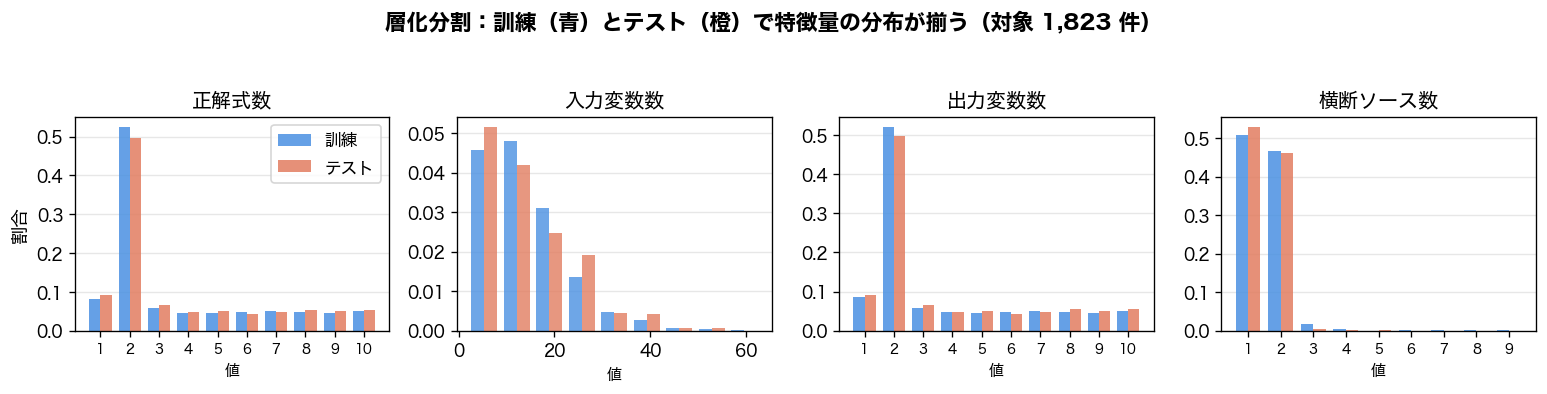
\includegraphics[width=\linewidth]{figures/fig_v6_splitbalance.png}
\caption{層化分割：訓練（青）とテスト（橙）で 4 つの特徴量の分布がそろう（対象 1{,}823 件、乱数 1 例）。}
\label{fig:split}
\end{figure}

%======================================================================
\section{テストケースの再生成（DAE）}\label{sec:dae}
%======================================================================
前のテストケースを調べると、\textbf{物理モデルを構成する数式が最大 4 式と少なく}、\textbf{代数方程式（時間微分を含まず、変数どうしの関係だけを表す等式。例：物質収支 $F_{\mathrm{in}}=F_{\mathrm{out}}$ や状態方程式 $PV=nRT$）が半数を占める}という偏りがあった。これでは物理モデルとして本来重要な「時間変化を表す常微分方程式（ODE）と、それに付随する代数方程式が連立する系（微分代数方程式系、DAE）」が十分に含まれない。そこで、\textbf{加藤先生にご指摘いただいた次の手順}でケースを作り直した（正解式数 $X=1,\dots,10$ について各 100 件、計 1{,}000 件）。

\begin{tcolorbox}[colback=gray!5, colframe=gray!50, boxrule=0.4pt, left=2mm, right=2mm, top=1mm, bottom=1mm]
\small
\begin{enumerate}[leftmargin=1.6em, nosep]
  \item[0.] $X$ を決める（$X\in\{1,2,\dots,10\}$）。
  \item いずれかのソースから微分方程式を見つけ、正解数式集合に加える。
  \item 微分方程式の左辺の微分されている変数を出力とする。
  \item 正解数式集合に含まれる「出力変数以外」の変数を含む数式を、同じソースか別のソースから見つけて加える。パラメータに代入するだけの数式（左辺が変数、右辺が数値）でもよい。
  \item 数式の数が $X$ になるまで 3 を繰り返す。$X$ が大きいとき無限ループにならないよう、全ソースを探索したら打ち切る。
  \item 正解数式集合に含まれる変数のうち、出力変数以外を入力変数とする。
  \item （正解数式集合、出力変数、入力変数）の組を正解とし、これらからモデルの説明文を作成する。
  \item 1--6 を、正解ケースが 100 件になるまで繰り返す。
\end{enumerate}
\end{tcolorbox}

たとえば、連続槽型反応器（CSTR；反応物を連続的に供給・排出しながら撹拌する槽）で槽内の反応物濃度 $C_A$（mol/m$^3$）の時間変化を求めるモデルは、次の 3 式を連立して初めて解ける。(i) 物質収支の常微分方程式 $V\,\mathrm{d}C_A/\mathrm{d}t = F\,(C_{A0}-C_A) - V\,r_A$（$V$：槽体積 m$^3$、$F$：流量 m$^3$/s、$C_{A0}$：入口濃度 mol/m$^3$、$r_A$：反応速度 mol/(m$^3\cdot$s)）、(ii) 反応速度式 $r_A = k\,C_A$（$k$：反応速度定数 1/s）、(iii) 反応速度定数の温度依存を表すアレニウスの式 $k = A\exp(-E/RT)$。手順 1 で (i) の ODE を出発点（種）とし、手順 3 で (ii)(iii) のように\textbf{変数を共有する式}（ここでは $r_A$ や $k$）を順に足していく。

この手順は \texttt{generate\_dae\_cases.py} に実装した。手順 6 の説明文生成のみ大規模言語モデル（Anthropic Claude）を用い、それ以外（ODE の探索・微分変数の抽出・変数を共有する式の追加）はすべて規則ベースで行う。生成時には、\textbf{未知数（出力変数）の個数を方程式の本数 $X$ に一致させ}（一致しないケースは捨てる）、残りの変数はすべて既知の入力変数とする。未知数と式数が等しい正方系なので、入力を与えれば解が一意に定まる（これを\textbf{自由度ゼロ}と呼ぶ）。こうして構成上\textbf{解ける DAE ケース}が得られる。

%======================================================================
\section{API による再現可能な実装}\label{sec:api}
%======================================================================
論文に載せる実験は、誰が再実行しても同じ結果になる必要がある。デスクトップ／Web アプリ（Claude や Gemini のアプリ）は、過去の対話ログを参照したり、内部の処理が予告なく変わったりするため、実験には使わない。本研究では LLM を使う部分（DAE ケースの説明文生成、および外部比較に用いる LLM 直接生成）を、すべて\textbf{API を呼ぶスクリプト}として実装した（\texttt{generate\_dae\_cases.py}、\texttt{evaluate\_llm\_dae.py}；モデルは日付指定版 \texttt{claude-sonnet-4-5-20250929}）。本手法（reranker）自体は LLM を使わない決定的な Python スクリプトであり、入力（説明文・入出力変数）を与えれば\textbf{第三者が同じ結果を再現できる}。

%======================================================================
\section{評価指標：Recall@3 から Recall@$K$ へ}\label{sec:metric}
%======================================================================
前回までは \textbf{Recall@3}（上位 3 件のうち正解式が占める割合）を主指標にしていた。しかし窓幅を 3 に固定すると、正解式が 4 件あるケースでは上位 3 件をすべて当てても $3/4$ までしか取れず、逆に正解式が 1 件のケースでは無関係な式を 2 件混ぜても満点になる。そこで、\textbf{窓幅をそのケースの正解式数 $K$ に合わせる Recall@$K$}に変えた。Recall@$K$ は「\textbf{必要な式を、過不足ない件数だけ上位にそろえられたか}」を、正解式数の多少によらず公平に測れる。たとえば Recall@$K=0.74$ は、必要な式のうち平均 74\% を上位 $K$ 件に正しく並べられたことを意味する。補助指標として MAP（平均適合率：正解の式をどれだけ上位にまとめられたかを表す指標）と、人手レビューを前提とした実用指標 Recall@20（上位 20 件に必要な式が入る割合）も併記する。

%======================================================================
\section{評価}\label{sec:eval}
%======================================================================

\subsection{実験設定（データ拡張の影響を除く）}\label{sec:setting}
データ拡張で水増ししたケース（単一文献の入出力を無作為に入れ替えた\textbf{無作為入替}ケースと、説明文を言い換えた\textbf{言い換え}ケース）を含めると、問題本来の難しさが薄まる。そこで影響を切り分けるため、次の 2 設定で評価した。いずれも \S\ref{sec:split} の層化分割・10 通りの乱数で評価する。

\begin{itemize}[leftmargin=1.5em]
  \item \textbf{設定 A}：拡張を除いた\textbf{原型}・\textbf{複数文献}・\textbf{DAE} のみ、計 \textbf{1{,}823 件}。
  \item \textbf{設定 B}：最も難しい \textbf{DAE} のみ、計 \textbf{1{,}000 件}。
\end{itemize}

比較対象は次の 3 つである。\textbf{baseline}（古典的情報検索：説明文と数式の文章類似度などで並べる第 1 段。特徴量は文章・変数の類似度など 7 個）、\textbf{reranker-10S}（本手法：第 1 段の候補を、数式グラフから作った\textbf{集合特徴量}も加えて並べ直す第 2 段）、そして外部手法の\textbf{LLM 直接生成}（説明文と入出力変数だけから LLM に必要な数式を生成させ、現行 DB と照合して順位付けする。本研究で LLM を解く側に使うのはこの比較のみ）である。ここで\textbf{集合特徴量}とは、各候補式を単独でなく\textbf{すでに選んだ式の集合との関係}で評価する量で、未充足の入力変数をどれだけ補えるか（補完性）・既選択集合と変数をどれだけ共有するか（一貫性）・同じ分野か（ドメイン一致）の 3 個からなる。名称の「10S」は、第 2 段で使う特徴量が計 10 個（基本 7 個＋集合特徴量〔英語で set-aware〕3 個）であることを表し、並べ直しには多層パーセプトロン（MLP）を用いる。

図~\ref{fig:aug} に 3 手法の Recall@$K$ を示す（LLM の生成は \texttt{claude-sonnet-4-5-20250929}、各設定の一様サンプル約 50 件）。\textbf{全設定で reranker（本手法）＞ baseline（古典 IR）＞ LLM 直接生成}である。LLM は表記が DB と異なっても物理的に等価なら正解とするよう、\textbf{生成式と正解式の等価性を別の大規模言語モデル（\texttt{claude-opus-4-8}）で判定}して採点したが、Recall@$K$ は $0.23$–$0.30$ にとどまる。ただし\textbf{LLM は等価な式を生成できてはおり}（順位を問わない coverage は $0.34$–$0.57$、図の破線）、それを\textbf{上位 $K$ 件に並べられないこと}、および DB の正解式に特定論文由来の経験式（特定の係数を含む式）が多く逐語生成が難しいことが、検索＋再順位付けに劣る主因である。古典 IR でも LLM 単独でも足りず、集合として並べ直す本手法が要ることを示す。

\noindent 同図はデータ拡張の影響も示す。拡張ケースも含めた\textbf{全 2{,}838 件のケースプール}に \S\ref{sec:split} と同じ層化分割（ソース単位 6:2:2・10 シード）を適用し、\textbf{テスト分割で}評価すると、baseline の Recall@$K$ は $0.622$ となり、拡張を除いた設定 A（$0.521$）より $0.101$ も高く出る。易しい拡張ケースが baseline を過大に見せるためで、本手法との差は\textbf{設定 A の $+0.222$ から、拡張込みでは $+0.156$ に縮んで見える}。すなわち拡張を残したまま評価すると、提案手法の効果を約 $0.07$ 過小評価してしまう。これが拡張を除く理由である。

\begin{figure}[h]\centering
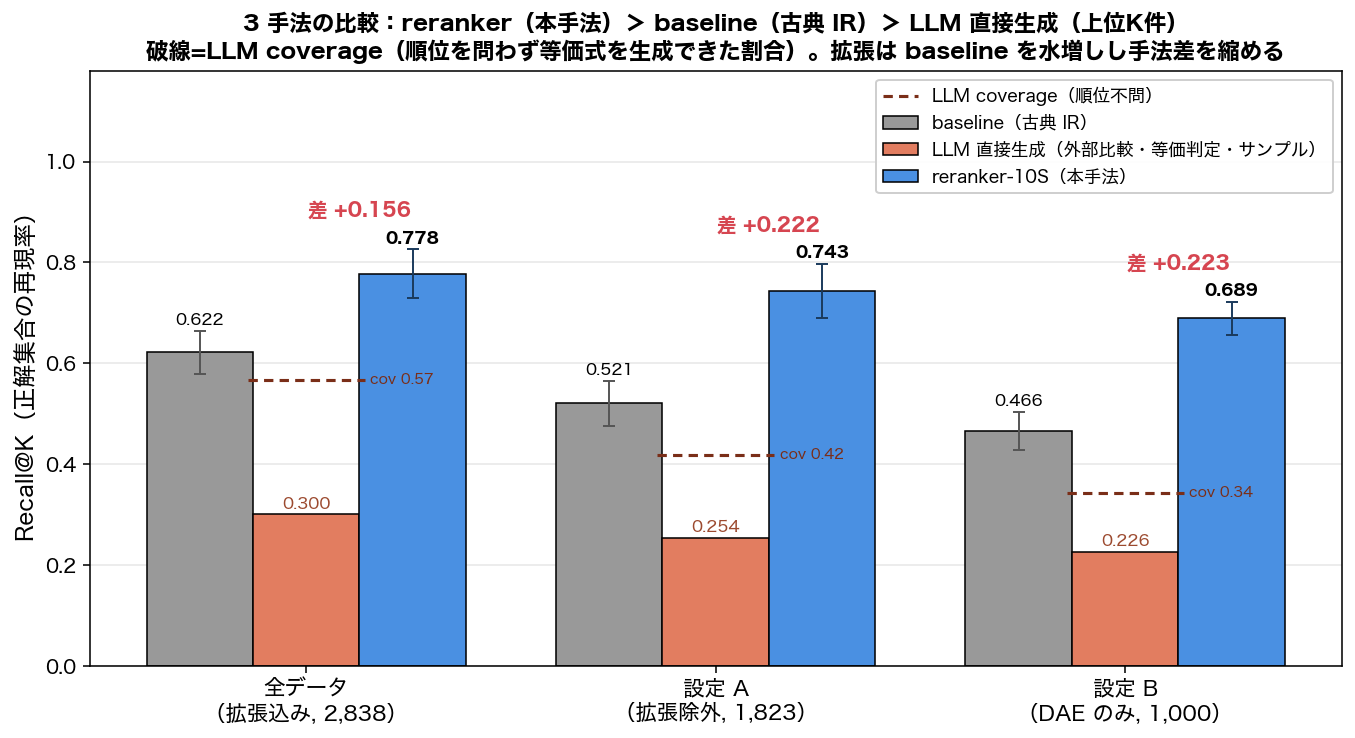
\includegraphics[width=\linewidth]{figures/fig_strat_augmentation.png}
\caption{3 手法の比較：全データ（拡張込み）・設定 A（拡張除外）・設定 B（DAE のみ）での baseline（古典 IR）・LLM 直接生成・本手法（reranker-10S）の Recall@$K$。全設定で reranker ＞ baseline ＞ LLM。baseline・本手法は 10 乱数の全件平均（エラーバー＝標準偏差）、\textbf{LLM は各設定の一様サンプル（$n\approx 50$）で、生成式の等価性を \texttt{claude-opus-4-8} で判定して採点}。\textbf{破線＝LLM の coverage}（順位を問わず等価式を生成できた割合）で、Recall@$K$ との差は「生成できるが上位 $K$ 件に並べられない」ことを表す。データ拡張は baseline を $+0.101$ 水増しし、本手法との差を $+0.222\to+0.156$ に縮める。}
\label{fig:aug}
\end{figure}

\subsection{全体の結果}\label{sec:overall}
表~\ref{tab:overall} に両設定の結果を示す。\textbf{本手法は両設定とも Recall@$K$ を $+0.22$ ポイント引き上げ}、必要な式集合のうち上位 $K$ 件に正しくそろう割合を、設定 A で $0.521\to0.743$（$+0.222$）、最難の設定 B でも $0.466\to0.689$（$+0.223$）に改善した。人手レビュー前提の Recall@20 は設定 A で $0.91$、DAE のみでも $0.84$ に達する。文章類似度だけの baseline では、複数の文献にまたがる式や変数の共有関係を捉えきれないことが、差にそのまま表れている。

\begin{table}[h]\centering
\small
\caption{層化分割・10 通りの乱数での平均（$\pm$ は乱数間の標準偏差）。本手法は両設定で Recall@$K$ を $+0.222$（設定 A）・$+0.223$（設定 B）改善する。}
\label{tab:overall}
\begin{tabular}{llccc}
\toprule
設定 & 手法 & Recall@$K$ & MAP & Recall@20 \\
\midrule
\multirow{2}{*}{A（原型＋複数文献＋DAE, 1{,}823 件)}
 & baseline & $0.521\pm0.045$ & $0.581$ & $0.836$ \\
 & \textbf{reranker-10S（本手法）} & $\mathbf{0.743\pm0.054}$ & $\mathbf{0.863}$ & $\mathbf{0.909}$ \\
\midrule
\multirow{2}{*}{B（DAE のみ, 1{,}000 件)}
 & baseline & $0.466\pm0.037$ & $0.512$ & $0.721$ \\
 & \textbf{reranker-10S（本手法）} & $\mathbf{0.689\pm0.033}$ & $\mathbf{0.832}$ & $\mathbf{0.838}$ \\
\bottomrule
\end{tabular}
\end{table}

\subsection{特性別の分析：どんなケースで性能が変わるか}\label{sec:char}
設定 A のケースごとの結果を、数式数・ソース数・入力変数数で層別した（図~\ref{fig:char}）。

\begin{itemize}[leftmargin=1.5em]
  \item \textbf{数式数（図 a）}：数式が多いほど難しくなる。baseline は正解式数が 1 のとき $0.85$ だが 10 では $0.28$ まで落ちる。本手法も $0.88\to0.54$ と下がるが落ち方は緩やかで、\textbf{差は単一式の $+0.03$ から複数式の $+0.21\sim+0.29$ へ広がる}。「易しい問題を壊さず、難しい組合せ問題で効く」という望ましい性質を示す。
  \item \textbf{入力変数数（図 c）}：入力変数が多いほど難しくなる。baseline は 5 個以下の $0.80$ から 21 個以上の $0.37$ へ落ちる一方、本手法は $0.85\to0.66$ にとどまり、\textbf{差は $+0.05$ から $+0.28$ へ広がる}。
  \item \textbf{ソース数（図 b）}：ソース数そのものは性能とほぼ無関係だった。これはソース数が数式数と交絡している（2 文献のケースの多くは 2 式の易しい問題）ためで、\textbf{本手法の優位はソース数によらず $+0.22\sim+0.26$ でほぼ一定}である。
\end{itemize}

\noindent まとめると、\textbf{数式数と入力変数数が増えるほど問題は難しくなり、そこでこそ本手法の上乗せが大きくなる}。出力変数数は正解式数とほぼ一致するため、数式数と同じ傾向を示す。

\begin{figure}[h]\centering
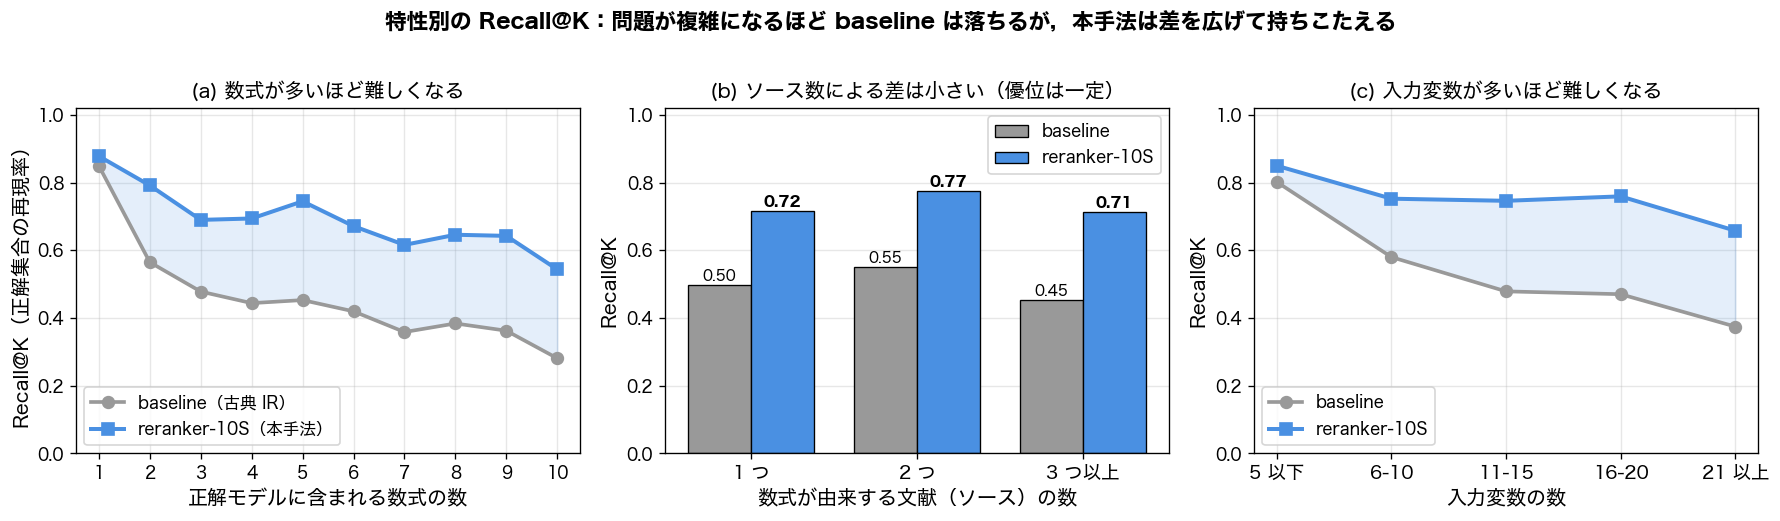
\includegraphics[width=\linewidth]{figures/fig_strat_characteristic.png}
\caption{特性別の Recall@$K$（設定 A、ケース単位を 10 乱数で平均）。(a) 数式数、(b) ソース数、(c) 入力変数数。問題が複雑になるほど baseline（灰）は落ちるが、本手法（青）は差を広げて持ちこたえる。}
\label{fig:char}
\end{figure}

\subsection{留意点}
本結果には次の前提がある。(1) DAE ケースの説明文は LLM が生成しており、表現の揺れを含む。(2) ソース数の効果は数式数と交絡しているため、単独の因果とは解釈できない。(3) 値は 10 通りの乱数分割の平均であり、層化分割は 400 候補から選んだ 1 つの方式である。

%======================================================================
\section{まとめと今後}
%======================================================================
\textbf{今回}：データベースを 11{,}146 式・2{,}838 件に拡大し、分布をそろえた層化分割と、加藤先生ご指摘の手順による DAE ケースの再生成を行い、API で再現可能な実験基盤を整えた。評価指標を Recall@$K$ に改めたうえで、データ拡張の影響を除いた 2 設定で評価した結果、\textbf{本手法は Recall@$K$ を $+0.22$ ポイント改善}（設定 A $+0.222$、設定 B $+0.223$）し、その効果は\textbf{数式数・入力変数数が多い難しいケースほど大きい}ことを特性別分析で確かめた。

\textbf{今後}：
\begin{itemize}[leftmargin=1.5em]
  \item PSE Asia 発表の準備（本報告のデータ拡大・層化分割・DAE 再生成・特性別評価を中核に据える）。
  \item 数式数・入力変数数が多いケースで性能が下がる問題に対し、手法を改善する。
  \item 論文執筆（API ベースの再現可能な実験一式を整備し、LLM 直接生成との同条件比較を DAE まで拡張する）。
\end{itemize}

\end{document}
